%% Canonical Neural Networks (Elsevier) manuscript
%% Based on official elsarticle-template-harv.tex (elsarticle 3.5)
%% Do not modify elsarticle.cls or elsarticle-harv.bst.
%% Scientific source: current Factorized FALI evidence base.

\documentclass[preprint,12pt,authoryear]{elsarticle}

\usepackage{amssymb}
\usepackage{amsmath}
\usepackage{graphicx}
\usepackage{booktabs}
\usepackage{multirow}
\usepackage{placeins}
\usepackage{url}
\usepackage{hyperref}

\journal{Neural Networks}

\begin{document}

\begin{frontmatter}

\title{FALI: Mechanistic Decomposition of Conditional Attention-Head Causal Usefulness}

\author[inst1]{Ronith Sharmila\corref{cor1}}
\ead{ronith.sharmila@swosu.edu}
\author[inst2]{Delen Dursun}
\ead{dursun.delen@okstate.edu}
\author[inst3]{Rupesh Agrawal}
\ead{rupesh.agrawal@nku.edu}
\cortext[cor1]{Corresponding author}

\affiliation[inst1]{organization={Southwestern Oklahoma State University},%
            city={Weatherford},
            country={USA}}

\affiliation[inst2]{organization={Oklahoma State University},%
            city={Stillwater},
            country={USA}}

\affiliation[inst3]{organization={Northern Kentucky University},%
            city={Highland Heights},
            state={Kentucky},
            country={USA}}

\begin{abstract}
Transformer components can become more or less causally useful after another circuit component is perturbed. Conditional importance detects this change but does not explain its mechanism. We introduce FALI (Factorized Attention-Level Intervention), an output-grounded counterfactual framework that decomposes the change in a selected attention head's causal usefulness into target, rival, and other attention-score contributions, value content, and surrounding-network context. Standard Owen attribution allocates interactions while reconciling the fine score decomposition with a coarse score/value/context game. Controlled synthetic systems and a randomly initialized transformer validate factor isolation, endpoint recovery, intervention isolation, and coarse--fine consistency. In GPT-2 Small on indirect object identification, L10H2 is positively recruited after primary Name Movers are ablated and shows a target-positive/rival-negative score decomposition; L10H10 shows similar attention adaptation without positive recruitment. A preregistered transfer test in Pythia-160M induction again finds positive recruitment, but the target and rival contributions reverse sign. Thus, the same high-level functional response can arise through different fine-grained mechanisms. FALI provides a mechanism-discrimination layer for selected conditionally important attention heads under explicit intervention semantics.
\end{abstract}

\begin{graphicalabstract}
%% Optional at submission; figure assets live under figures/.
\end{graphicalabstract}

%% Research highlights (also in standalone highlights.tex)
\begin{highlights}
\item FALI decomposes conditional causal usefulness of selected attention heads.
\item GPT-2 IOI shows target-positive and rival-negative fine-score channels.
\item Pythia induction reverses the preregistered target/rival fine signs.
\item Positive recruitment recurs while the tested fine mechanism does not transfer.
\item FALI discriminates mechanisms under an explicit intervention game.

\end{highlights}

\begin{keyword}
mechanistic interpretability \sep causal intervention \sep transformer circuits \sep
attention heads \sep conditional importance \sep FALI
\end{keyword}

\end{frontmatter}

\section{Introduction}\label{sec:intro}

A transformer's internal components need not retain the same causal role after the circuit around them is perturbed. Ablating one component can change the contribution of others, producing self-repair, backup behavior, or more general conditional importance \citep{mcgrath2023hydra,mcdougall2023copysuppression,rushing2024selfrepair,gong2026coax}. Detecting such a change is useful, but it leaves a mechanistic question unresolved: \emph{why did the selected component become more or less useful?}

For an attention head, several explanations are possible. Its task-relevant attention score may increase; competing scores may decrease; value content may change; or essentially the same head output may become more or less useful because the surrounding network has changed. These possibilities are not interchangeable. A visible increase in attention can occur without positive functional recruitment, and two heads that satisfy the same conditional-recruitment criterion can in principle do so through different internal changes.

We introduce \textbf{FALI (Factorized Attention-Level Intervention)}, a hypothesis-driven framework for resolving that ambiguity. FALI starts after a candidate attention head and a task-relevant target edge have been identified. It compares an intact state with a perturbed state and decomposes the resulting change in the candidate's \emph{output-grounded causal usefulness}. The candidate's attention computation is factorized into target scores $T$, rival scores $R$, other valid scores $O$, value content $V$, and surrounding-network context $C$. Evaluating the resulting $2^5$ counterfactual states defines a causal game whose interactions are allocated with the standard Owen value. The fine score contributions reconcile exactly with a coarser SCORE/VALUE/CONTEXT decomposition.

The key distinction is between \emph{localizing conditional importance} and \emph{explaining it}. Path and activation patching identify behaviorally relevant components or paths \citep{goldowskydill2023pathpatching,zhang2024activationpatching,heimersheim2024activationpatching}; conditional co-ablation identifies components whose importance changes after a primary intervention \citep{gong2026coax}; interaction-aware mediation analyses show that a component's measured effect can depend strongly on the rest of the model \citep{vaidyanathan2026curse}. FALI is downstream of these approaches: given a selected conditional change, it asks which architecture-aligned changes account for it under an explicit intervention model.

We first validate the intervention semantics in controlled systems. Deterministic synthetic attention models isolate each of $T,R,O,V,C$ and a known cross-factor interaction, while a small randomly initialized transformer checks score-to-pattern reconstruction, value-to-output reconstruction, endpoint recovery, intervention isolation, batch-specific score partitions, and consistency between the fine Owen game and its coarse quotient game. These tests establish that the implementation recovers the factors it manipulates; they do not claim that the factorization is unique or that hybrid states are naturally occurring model states.

We then apply FALI to GPT-2 Small on indirect object identification (IOI) \citep{wang2023ioi}. Corrected functional analysis separates attention adaptation from recruitment: after the canonical primary Name Movers are removed, L10H2 becomes more causally useful, whereas L10H10 increases target attention even more strongly while its causal usefulness decreases. FALI assigns both heads a target-positive/rival-negative score pattern, showing that even a seemingly favorable score reorganization does not itself define recruitment. For positively recruited L10H2, the main fine-score contributions are $\phi_T>0$ and $\phi_R<0$ across the canonical confirmation cohort.

The decisive test is cross-setting transfer. We prospectively test the GPT-2 target-positive/rival-negative mechanism in Pythia-160M induction. Positive conditional recruitment appears again, but the fine score signs reverse: $\phi_T<0$ and $\phi_R>0$. Thus the preregistered mechanism-transfer hypothesis fails. The shared functional label---conditional recruitment---does not imply a shared fine-grained mechanism.

Our contributions are threefold. First, we define an output-grounded counterfactual estimand for the cross-state change in a selected attention head's causal usefulness. Second, we factor that change into score, value, and surrounding-context contributions, with target/rival/other resolution inside SCORE and coarse--fine consistency via standard Owen attribution. Third, we show empirically that two settings with positive conditional recruitment can exhibit opposite target/rival score mechanisms. To our knowledge, this combination provides a distinct mechanism-resolution layer for conditionally important attention heads, rather than a new theory of self-repair, a new circuit-discovery method, or new Shapley/Owen mathematics.

\section{Related Work}\label{sec:related}

\subsection{Self-repair and conditional component importance}\label{sec:rw-conditional}

Transformer circuits can adapt when components are ablated. The IOI circuit analysis of \citet{wang2023ioi} identified primary and backup Name Mover heads in GPT-2 Small, providing an early concrete setting in which several attention heads participate in a behavior and some become especially relevant under intervention. Recent prompt-specific circuit work further shows that mechanisms can vary systematically across templates even within IOI, reinforcing the need to state the distribution over which a mechanistic claim is supported \citep{franco2026promptspecific}. Subsequent work established self-repair more broadly. The Hydra effect describes compensatory changes in downstream language-model computation after ablation \citep{mcgrath2023hydra}. Copy-suppression analysis showed that self-repair can arise through specific functional mechanisms rather than a single generic backup process \citep{mcdougall2023copysuppression}. \citet{rushing2024selfrepair} further found self-repair across model families and the full training distribution, with substantial prompt-level variability and contributions from mechanisms including LayerNorm scaling and anti-erasure.

FALI does not claim the discovery of self-repair or heterogeneous compensation. More directly, it also does not introduce the idea of conditional component importance. \citet{gong2026coax} formalize Conditional Co-Ablation (CoAx), which scores how much a remaining unit's ablation effect grows once a primary set has been removed. Their experiments show that this conditional score can recover backup heads missed by first-order rankings and transfers from GPT-2 IOI to induction settings across multiple models. This establishes both the empirical relevance and the practical utility of asking how component importance changes under intervention.

The distinction is therefore one of explanatory stage. Conditional ablation answers whether, or to what extent, a component becomes more important in a perturbed circuit. FALI assumes such a candidate has already been selected and asks which changes in the candidate's attention-score computation, value content, and surrounding context account for that cross-state change. In this sense CoAx and FALI are complementary: the former can identify \emph{which} components warrant conditional analysis, whereas FALI provides a structured mechanism-resolution experiment for a chosen attention head.

\subsection{Interaction-aware causal attribution}\label{sec:rw-interaction}

Activation patching and related interchange interventions are standard tools for testing whether internal activations causally contribute to model behavior. Path patching refines this idea to hypotheses about particular computational paths \citep{goldowskydill2023pathpatching}; systematic studies have also shown that patching conclusions depend on choices such as corruption, metric, and intervention design \citep{zhang2024activationpatching,heimersheim2024activationpatching}. These methods are primarily localization or causal-testing tools: they identify components, activations, or paths whose replacement changes an outcome. FALI uses the same broad experimental tradition but addresses a different estimand---the change in one selected head's output-grounded causal contribution between two circuit states.

A particularly close conceptual neighbor is \citet{vaidyanathan2026curse}. Re-deriving activation patching through causal mediation analysis, they show that a component's natural indirect effect can include interaction terms that measure how its effect depends on the state of other model components. In GPT-2 IOI these interactions can hide conditionally important components, inflate others, and contribute to instability in component rankings. This result rules out any novelty claim that FALI is the first method to observe context-dependent causal effects. Instead, it motivates the next question: once a conditional or interaction-dependent effect has been identified, can we resolve that change into architecture-level factors of the selected attention head?

Causal Head Gating provides a complementary head-level perspective. \citet{nam2025causalhead} learn gates over attention heads, classify their roles as facilitating, interfering, or irrelevant, and find that head roles can depend on interactions with other heads. FALI is neither a learned gating method nor a global head-role taxonomy. It fixes one candidate head and two model states, then intervenes on explicitly defined internal factors of that head and the surrounding model. Likewise, we do not claim that FALI is generally more faithful than patching: intervention-based interpretability results can be sensitive to methodology, as demonstrated by circuit-faithfulness studies \citep{miller2024faithfulness}. Our robustness experiments therefore support only the intervention variants actually tested.

These interaction-aware results also inform our interpretation of the context factor $C$. Under FALI, $C$ is not a localized ``downstream sensitivity'' variable. It denotes the surrounding model computation that differs between intact and perturbed contexts outside the explicitly injected candidate score/value state. It can therefore aggregate changes in other heads, MLPs, residual representations, normalization, and upstream or downstream computation. A large $\phi_C$ is evidence about the specified counterfactual game, not identification of a unique external mechanism.

\subsection{Decomposing attention computation}\label{sec:rw-attention}

The separation between attention routing and transported content is foundational rather than novel to FALI. The transformer-circuits framework distinguishes the query--key (QK) circuit, which determines attention scores and patterns, from the output/value (OV) circuit, which determines what information is written when a source position is attended to \citep{elhage2021mathematical}. Later causal work makes increasingly fine distinctions inside attention computation. \citet{franco2025attentioncausal} identify low-dimensional communication signals with a causal relationship to attention patterns, while \citet{wang2026fewshot} causally separate Query--Key routing from Value updates when explaining how few-shot examples shape function vectors. Recent factorial intervention work likewise shows that attention allocation and token content can be experimentally separated yet strongly coupled in a different robustness setting \citep{zhu2026lexical}.

FALI builds on these distinctions but changes the object being decomposed. Its dependent quantity is not the attention pattern itself, nor the quality of a function vector, but the \emph{cross-state change in the selected head's downstream causal usefulness}. SCORE and VALUE are therefore accompanied by an explicit CONTEXT factor. Within SCORE, FALI further partitions structurally valid score coordinates into task-target scores $T$, rival scores $R$ in the same task-relevant query row, and all other valid scores $O$. This target/rival/other partition is hypothesis-driven: it requires a task-relevant target edge or edge set to be specified in advance, and is not an automatic circuit-discovery procedure.

Because score, value, and context can interact non-additively, FALI uses the standard Owen value for a game with a priori coalition structure \citep{owen1977values}. The coalition structure is fixed as SCORE=$\{T,R,O\}$, VALUE=$\{V\}$, and CONTEXT=$\{C\}$. Owen attribution is established game-theoretic machinery; our use of it is motivated by the requirement that the fine score contributions reconcile with the coarse SCORE contribution rather than by a claim of a new attribution theorem. The resulting values should also be read relative to the intervention semantics. Hybrid internal states need not be states the unmodified model would naturally visit, and causal-intervention research has documented that representation-level interventions can move models away from their natural internal distributions \citep{grant2025divergent}. We therefore treat FALI as a controlled counterfactual decomposition, not as evidence that the model implements five independent natural pathways.

Finally, our emphasis on explicit validation reflects a broader evaluation problem in mechanistic interpretability. Benchmarks such as MIB prioritize precise recovery of causal pathways or variables rather than plausible narrative alone \citep{mueller2025mib}. FALI's synthetic single-factor systems and implementation invariants serve the narrower purpose of checking that the intervention pipeline recovers known manipulated factors before empirical use. They do not remove the substantive limitations of target selection, coalition choice, or intervention dependence, which we address explicitly in Section~\ref{sec:limitations}.

An earlier public preprint introduced the name FALI for \emph{Frozen Attention Logit Intervention} and analyzed target-versus-background attention-logit changes in GPT-2 IOI \citep{sharmila2026attentionrepairs}. The present work supersedes that attention-probability interpretation. It changes the estimand to output-grounded conditional causal usefulness; expands the intervention game to $T/R/O/V/C$; uses standard Owen attribution with coarse--fine reconciliation; adds controlled implementation validation and broad canonical confirmation; and includes a prospectively frozen cross-setting transfer test whose fine-mechanism hypothesis fails. We therefore treat the earlier method as a nested attention-probability special case rather than as evidence for the present causal mechanism claims.

\section{Problem Formulation}\label{sec:problem}

\subsection{Conditional causal usefulness}\label{sec:conditional-usefulness}

Let $f$ be a transformer evaluated by a scalar task metric $m$. We consider two executions of the same task instance: an \emph{intact} state $A$ and a \emph{perturbed} state $B$, obtained by applying a prespecified intervention to a primary circuit component or set of components. Let $h$ denote a candidate attention head whose change in functional importance we want to explain. The task metric can differ across applications---for example, an IO-minus-subject logit difference in IOI or the target-token log probability in induction---but it is fixed within an analysis.

For context $s\in\{A,B\}$, let $m_s^{h}$ be the task metric with the candidate head operating normally and let $m_s^{0}$ be the metric when that candidate is zeroed while all other aspects of context $s$ are held fixed. We define the candidate's output-grounded causal usefulness in context $s$ as
\begin{equation}
E_s(h) = m_s^{h}-m_s^{0}.
\label{eq:context-effect}
\end{equation}
The intact and conditional effects are therefore $E_A(h)$ and $E_B(h)$, respectively. The cross-state change we seek to explain is
\begin{equation}
\Delta_h = E_B(h)-E_A(h).
\label{eq:conditional-gain}
\end{equation}
In our experiments this quantity is called \emph{conditional gain}. Positive $\Delta_h$ means that the candidate's contribution becomes more positive after the primary intervention; it does not by itself imply that the candidate is supportive in the perturbed state. We reserve \emph{positive functional recruitment} for cases in which both $E_B(h)>0$ and $\Delta_h>0$. FALI itself is not restricted to positive recruitment: it decomposes positive or negative changes in causal usefulness.

This definition deliberately evaluates the candidate against a zero-candidate baseline in the \emph{same} surrounding context. Consequently, a difference between $E_A(h)$ and $E_B(h)$ cannot be produced merely by a shift in the task metric that affects both the candidate-present and candidate-zero conditions equally. The estimand is the change in the candidate's marginal causal contribution under the specified intervention, not the raw performance difference between states $A$ and $B$.

\subsection{Mechanism-resolution objective}\label{sec:mechanism-objective}

The problem begins after a candidate head and a task-relevant attention target have been chosen. They may come from prior circuit analysis, conditional co-ablation, patching, or a task-specific hypothesis. FALI does not search over heads, discover a target edge, or infer a circuit automatically. Its input is a selected head $h$, two model states $A$ and $B$, a scalar task metric $m$, and a target query--key edge (or prespecified target edge set) whose score is meaningful for the task.

The objective is to account for $\Delta_h$ using changes in three architecture-level objects associated with the candidate: its pre-softmax attention scores, its value vectors, and the surrounding computation in which the resulting head output is used. The score tensor is then resolved more finely into the task-target score, rivals in the same query row, and scores at other query positions. This yields a controlled mechanism-discrimination question: under a fixed intervention algebra, which candidate-local or surrounding changes receive credit for the observed change in output-grounded usefulness? Figure~\ref{fig:fali-overview} summarizes this distinction.

\begin{figure*}[t]
\centering
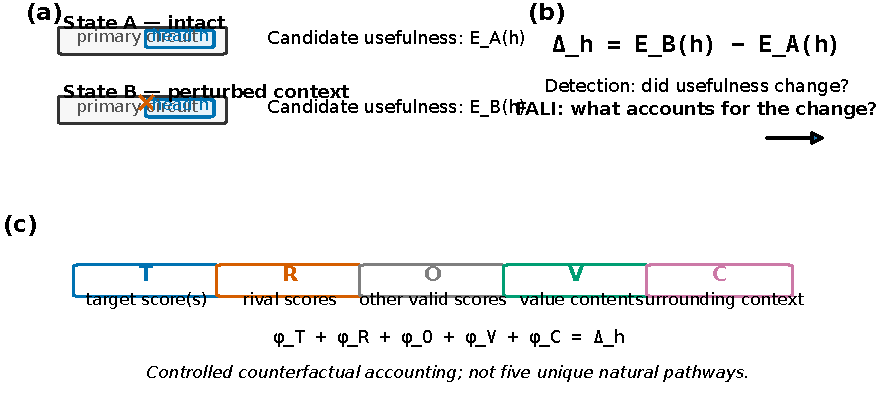
\includegraphics[width=\textwidth]{figures/Fig1.pdf}
\caption{\textbf{FALI resolves a conditional change in a selected attention head's causal usefulness.}
(a) The same candidate head $h$ is evaluated in an intact state $A$ and a prespecified perturbed state $B$.
(b) The quantity to be explained is the cross-state change $\Delta_h=E_B(h)-E_A(h)$ in output-grounded causal usefulness.
(c) FALI attributes this endpoint change under an explicit intervention game across task-target scores ($T$), rival scores ($R$), other structurally valid scores ($O$), value content ($V$), and surrounding-network context ($C$), with Owen efficiency $\phi_T+\phi_R+\phi_O+\phi_V+\phi_C=\Delta_h$.
The candidate head and task-relevant target coordinates are specified before FALI analysis.}
\label{fig:fali-overview}
\end{figure*}


\section{Factorized Attention-Level Intervention}\label{sec:fali}

\subsection{Architecture-aligned factors}\label{sec:factors}

For one candidate head and one task instance, let $S^{A}$ and $S^{B}$ denote its cached pre-softmax attention-score tensors in the intact and perturbed executions, and let $V^{A}$ and $V^{B}$ denote its corresponding value tensors. Let $q^{\star}$ be the task-relevant query position and $k^{\star}$ the target key position. We use an explicit structural validity mask
\begin{equation}
\mathcal{M}=\{(q,k): q<\ell,\; k\le q\},
\label{eq:valid-mask}
\end{equation}
for a right-padded causal sequence of valid length $\ell$; padding and future positions are structural constants rather than intervention variables. The valid score coordinates are partitioned into
\begin{align}
T &= \{(q^{\star},k^{\star})\}, \\
R &= \{(q^{\star},k)\in\mathcal{M}: k\neq k^{\star}\}, \\
O &= \mathcal{M}\setminus (T\cup R).
\label{eq:tro-partition}
\end{align}
Thus $T$, $R$, and $O$ are pairwise disjoint and cover every structurally valid score coordinate exactly once. When an application specifies multiple target edges, $T$ can be generalized to that prespecified set and $R$ defined as the remaining valid coordinates in the corresponding task-relevant query row(s); the experiments in this paper use one target coordinate per example.

FALI has five binary factors, each taking its value from state $A$ (coded 0) or state $B$ (coded 1):
\begin{itemize}
    \item $T$: task-target attention score(s);
    \item $R$: rival scores in the same task-relevant query row;
    \item $O$: all other structurally valid scores of the candidate head;
    \item $V$: candidate value vectors at all valid source positions;
    \item $C$: surrounding-network context, intact versus perturbed.
\end{itemize}
The first three factors jointly determine the complete candidate attention pattern. $V$ controls the content combined by that pattern. $C$ controls the rest of the model execution outside the explicitly injected candidate state. In particular, $C$ is not defined as a uniquely localized downstream mechanism; it can aggregate differences in other attention heads, MLPs, residual representations, normalization, and upstream or downstream computation.

\subsection{Counterfactual intervention game}\label{sec:game}

Let $(\tau,\rho,\omega,\nu,c)\in\{0,1\}^{5}$ denote one FALI cell. For a binary state index $b$, write $S^{b}=S^{A}$ if $b=0$ and $S^{b}=S^{B}$ if $b=1$, with the analogous convention for $V^{b}$. We construct a hybrid score tensor by taking each coordinate block from its selected endpoint,
\begin{equation}
S_{\tau\rho\omega}
=
\mathbf{1}_{T}\odot S^{\tau}
+\mathbf{1}_{R}\odot S^{\rho}
+\mathbf{1}_{O}\odot S^{\omega},
\label{eq:hybrid-scores}
\end{equation}
with invalid coordinates fixed to the structural attention mask. We then recompute the attention pattern from the hybrid scores,
\begin{equation}
P_{\tau\rho\omega}
=\operatorname{masked\_softmax}(S_{\tau\rho\omega}),
\label{eq:hybrid-pattern}
\end{equation}
and reconstruct the candidate head output using the selected value tensor,
\begin{equation}
z_{\tau\rho\omega\nu}[q]
=\sum_{k}P_{\tau\rho\omega}[q,k]V^{\nu}[k].
\label{eq:hybrid-z}
\end{equation}
The reconstructed $z$ is injected for the candidate head at all valid query positions. This full-output overwrite is important: the live candidate computation is not allowed to leak into a hybrid cell.

Let $F_c[z_h\leftarrow z]$ denote a forward pass in surrounding context $c$, with $c=0$ selecting state $A$ and $c=1$ selecting state $B$, and with the full output of candidate head $h$ replaced by $z$. The FALI utility for a cell is
\begin{equation}
U(\tau,\rho,\omega,\nu,c)
=
 m\!\left(F_c[z_h\leftarrow z_{\tau\rho\omega\nu}]\right)
-
 m\!\left(F_c[z_h\leftarrow 0]\right).
\label{eq:fali-utility}
\end{equation}
The zero-candidate comparison is always evaluated in the same context $c$ as the hybrid injection. FALI therefore contains $2^5=32$ counterfactual cells.

The two complete endpoints recover the effects in Eq.~\ref{eq:context-effect}:
\begin{align}
U(0,0,0,0,0) &= E_A(h), \\
U(1,1,1,1,1) &= E_B(h),
\end{align}
so that
\begin{equation}
\Delta_h
=U(1,1,1,1,1)-U(0,0,0,0,0).
\label{eq:fali-endpoint-identity}
\end{equation}
This endpoint identity is a required implementation invariant, not an approximation in the mathematical definition.

Most mixed cells need not correspond to an activation state encountered during an unmodified forward pass. FALI should therefore be read as an explicit counterfactual/interchange-intervention game. Its attributions are conditional on the chosen endpoint states, target partition, masking semantics, and intervention construction; they are not claims that the model naturally executes five separable causal pathways. Figure~\ref{fig:fali-game} depicts the 32-cell construction.

\begin{figure*}[t]
\centering
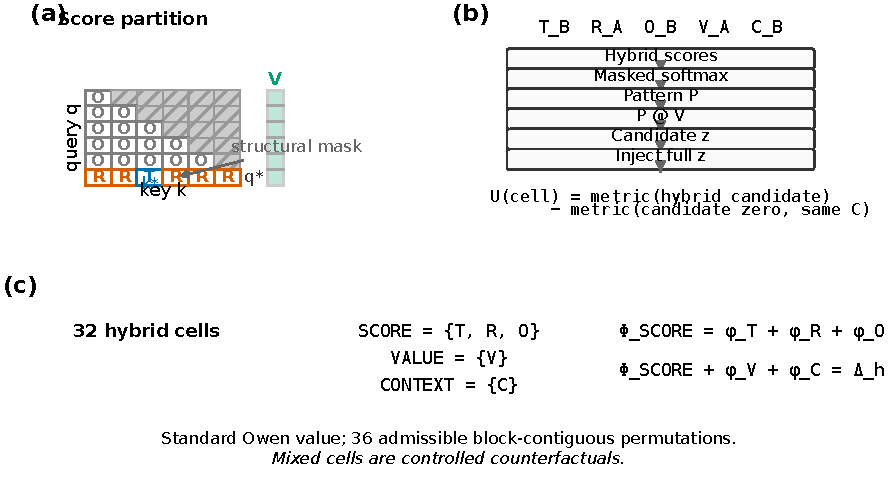
\includegraphics[width=\textwidth]{figures/Fig2.pdf}
\caption{\textbf{FALI constructs a 32-cell counterfactual intervention game for the selected attention head.}
(a) Structurally valid pre-softmax scores are partitioned into the prespecified task-target coordinate(s) $T$, rival scores $R$ in the same task-relevant query row, and all other valid scores $O$; masked coordinates are not players.
(b) Each hybrid cell selects $T,R,O,V,$ and $C$ from the intact or perturbed endpoint, reconstructs the candidate attention pattern and head output, and defines utility relative to a candidate-zero run in the same surrounding context $C$.
(c) All $2^5=32$ hybrid states are evaluated. Standard Owen attribution under $\mathrm{SCORE}=\{T,R,O\}$, $\mathrm{VALUE}=\{V\}$, and $\mathrm{CONTEXT}=\{C\}$ allocates the endpoint change over 36 block-contiguous admissible permutations, satisfying $\sum_i\phi_i=\Delta_h$ and $\Phi_{\mathrm{SCORE}}=\phi_T+\phi_R+\phi_O$.
The mixed cells are controlled counterfactual states, not claims that the model naturally implements five independent causal pathways.}
\label{fig:fali-game}
\end{figure*}


\subsection{Standard Owen attribution and coarse--fine reconciliation}\label{sec:owen}

Let the player set be $N=\{T,R,O,V,C\}$ and associate each coalition $K\subseteq N$ with the cell in which factors in $K$ take their $B$ state and all remaining factors take their $A$ state. This defines the characteristic function
\begin{equation}
v(K)=U(\mathbf{1}_{K}).
\label{eq:characteristic-game}
\end{equation}
Because the score factors are subdivisions of one computational object, whereas value and context are separate coarse factors, we fix the coalition structure
\begin{equation}
\Pi=\{\mathrm{SCORE}=\{T,R,O\},\;\mathrm{VALUE}=\{V\},\;\mathrm{CONTEXT}=\{C\}\}.
\label{eq:owen-partition}
\end{equation}
The partition membership is fixed; the block order is not. We use the standard Owen value, which averages marginal contributions over all permutations in which members of each block remain contiguous \citep{owen1977values}. For this partition there are $3!\times3!=36$ admissible permutations.

For completeness, let $G\in\Pi$ be the block containing player $i$, let $M=|\Pi|=3$, let $\mathcal{B}\subseteq\Pi\setminus\{G\}$ be a subset of predecessor blocks, and let $A_i\subseteq G\setminus\{i\}$ be a subset of predecessor players within $G$. Define $W_{\mathcal{B}}=\bigcup_{H\in\mathcal{B}}H$. The Owen value is
\begin{align}
\phi_i
={}&\sum_{\mathcal{B}\subseteq\Pi\setminus\{G\}}
\frac{|\mathcal{B}|!\,(M-|\mathcal{B}|-1)!}{M!}
\sum_{A_i\subseteq G\setminus\{i\}}
\frac{|A_i|!\,(|G|-|A_i|-1)!}{|G|!} \\
&\quad\times\left[
 v(W_{\mathcal{B}}\cup A_i\cup\{i\})
-v(W_{\mathcal{B}}\cup A_i)
\right].
\label{eq:owen-value}
\end{align}
This is equivalent to averaging sequential marginal contributions over the 36 admissible permutations. We use independent subset-weight and permutation implementations in validation.

The first property needed for interpretation is efficiency:
\begin{equation}
\phi_T+\phi_R+\phi_O+\phi_V+\phi_C
= v(N)-v(\varnothing)
=\Delta_h.
\label{eq:owen-efficiency}
\end{equation}
The attributions therefore allocate the entire endpoint change in causal usefulness, including interaction effects, under the specified game. They should not be interpreted as pure direct effects.

The second property gives the coarse--fine bridge. Define the quotient game on the three meta-players by
\begin{equation}
q(\mathcal{K})=v\!\left(\bigcup_{G\in\mathcal{K}}G\right),
\qquad \mathcal{K}\subseteq\Pi.
\label{eq:quotient-game}
\end{equation}
Standard Owen group consistency gives
\begin{align}
\Phi_{\mathrm{SCORE}}
&=\phi_T+\phi_R+\phi_O
=\operatorname{Shapley}_{q}(\mathrm{SCORE}), \\
\phi_V&=\operatorname{Shapley}_{q}(\mathrm{VALUE}), \\
\phi_C&=\operatorname{Shapley}_{q}(\mathrm{CONTEXT}).
\label{eq:quotient-consistency}
\end{align}
When the whole SCORE block switches together, its hybrid scores reproduce the complete $A$ or $B$ candidate pattern. The quotient SCORE/V/C game therefore matches the earlier pattern/value/context intervention game at the corresponding cells; this numerical bridge is tested explicitly in Section~\ref{sec:implementation-validation}. The purpose of Owen attribution here is not mathematical novelty but consistency between a coarse score/value/context explanation and the finer $T/R/O$ explanation inside SCORE.

Finally, the historical two-factor attention-probability version of FALI is nested as a special case rather than identified with the present causal attributions. If the utility is changed from output-grounded usefulness to target attention probability, $O$, $V$, and $C$ are held fixed, and only $T$ and $R$ vary, Eq.~\ref{eq:owen-value} reduces to the ordinary two-player Shapley decomposition of target-score versus competing-score changes. The present method changes both the intervention scope and, crucially, the quantity being explained.

\section{Method Validation}\label{sec:validation}

Before applying FALI to pretrained models, we tested whether the intervention game recovers known factors in controlled systems and reproduces ordinary transformer computation at its natural endpoints. These checks validate implementation semantics, not learned-model mechanisms. Figure~\ref{fig:validation} summarizes the main results; exact values and the validation chronology are provided in the Supplementary Information.

\begin{figure*}[t]
\centering
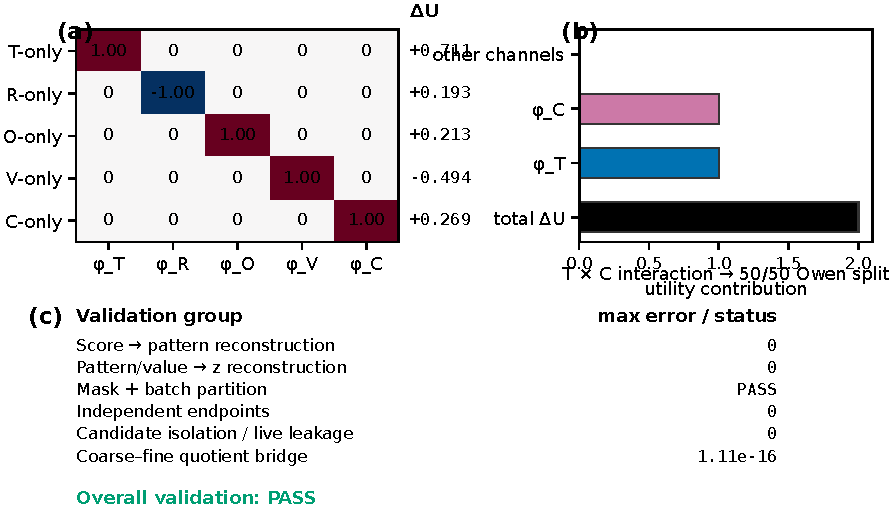
\includegraphics[width=\textwidth]{figures/Fig3.pdf}
\caption{\textbf{Controlled validation recovers known factors, interaction allocation, and transformer endpoint identities.}
(a) In five deterministic single-factor systems, the manipulated factor receives the full endpoint change: each row shows the recovery ratio $\phi_j/\Delta U_i$, with the raw injected $\Delta U_i$ given beside the row. The maximum attribution discrepancy is $1.11\times10^{-16}$.
(b) A pure $T\times C$ construction with $\Delta U\approx2$ yields the analytically expected Owen split $\phi_T\approx1$ and $\phi_C\approx1$, with $R,O,V=0$.
(c) In the randomly initialized two-layer TransformerLens validation model, independently measured intact effect, conditional effect, and conditional gain are $0.455046$, $-0.085684$, and $-0.540729$, respectively, and the corresponding FALI endpoint cells reproduce them exactly at recorded precision. Reconstruction, leakage, and model-level quotient residuals are zero at recorded precision.
These are implementation and controlled-ground-truth checks, not evidence that mixed FALI hybrids are unique natural model pathways.}
\label{fig:validation}
\end{figure*}


\subsection{Synthetic ground truth}\label{sec:synthetic}

We constructed deterministic attention systems containing masked softmax, values, $z=PV$, and a context-specific readout, then evaluated all 32 FALI cells. In five single-factor systems, only the manipulated factor received attribution up to floating-point precision. A separate pure $T\times C$ interaction produced the analytically expected equal Owen allocation between $T$ and $C$, with the remaining factors at zero. The all-intact and all-perturbed hybrids reconstructed their endpoints exactly at recorded precision, and collapsing $T,R,O$ into SCORE reproduced the corresponding SCORE/VALUE/CONTEXT quotient game with maximum discrepancy $1.11\times10^{-16}$.

\subsection{Transformer implementation invariants}\label{sec:implementation-validation}

We then repeated the mechanical checks in a randomly initialized two-layer TransformerLens model. Masked softmax reconstructed the cached attention patterns, pattern--value multiplication reconstructed the candidate head output, batch-specific $T/R/O$ masks formed a complete non-overlapping partition of valid scores, and candidate-output injection prevented live candidate computation from leaking into hybrid cells.

Independent ordinary forward passes gave intact effect $0.455046$, conditional effect $-0.085684$, and conditional gain $-0.540729$; the corresponding FALI endpoints reproduced all three with zero recorded discrepancy. Non-candidate heads remained unchanged under candidate-output overwrite, and the fine game agreed exactly with the collapsed SCORE/VALUE/CONTEXT quotient game.

Together, these tests establish factor isolation, structural masking, endpoint recovery, intervention isolation, and coarse--fine reconciliation for the implemented pipeline. They do not establish that the factorization is unique, that hybrid states lie on the model's natural activation manifold, or that a large attribution identifies a unique natural pathway.

\section{GPT-2 IOI: Recruitment and Mechanism}\label{sec:gpt2}

\subsection{Does attention increase imply recruitment?}\label{sec:gpt2-functional}

We apply FALI to GPT-2 Small on indirect object identification (IOI), perturbing the canonical primary Name Movers L9H6, L9H9, and L10H0 and using final-position IO-minus-subject logit difference as the task metric \citep{wang2023ioi}. The canonical confirmation cohort contains 15 low-level templates crossed with BABA/ABBA structure, 30 prompts per stratum, and four seeds, for 3600 prompts total. L10H2 and L10H10 are the primary candidate heads; L9H7 and L9H0 serve as same-layer architectural controls. Full sampling and bootstrap details are given in the Supplementary Information.

L10H2 satisfies the positive-recruitment criterion on the broad canonical cohort. Its conditional effect is $0.382$ (95\% CI $[0.341,0.424]$) and its conditional gain is $0.298$ ($[0.263,0.335]$). Its target attention also increases by $0.279$ ($[0.262,0.296]$).

L10H10 shows why attention adaptation is not sufficient evidence of recruitment. Its target attention increases even more, by $0.310$ ($[0.285,0.335]$), yet its conditional gain is negative, $-0.263$ ($[-0.302,-0.225]$), and its conditional effect is also negative, $-0.079$ ($[-0.111,-0.046]$). Figure~\ref{fig:gpt2-attention-recruitment}a therefore separates a visible attention response from the output-grounded functional response that FALI is designed to explain.

\begin{figure*}[t]
\centering
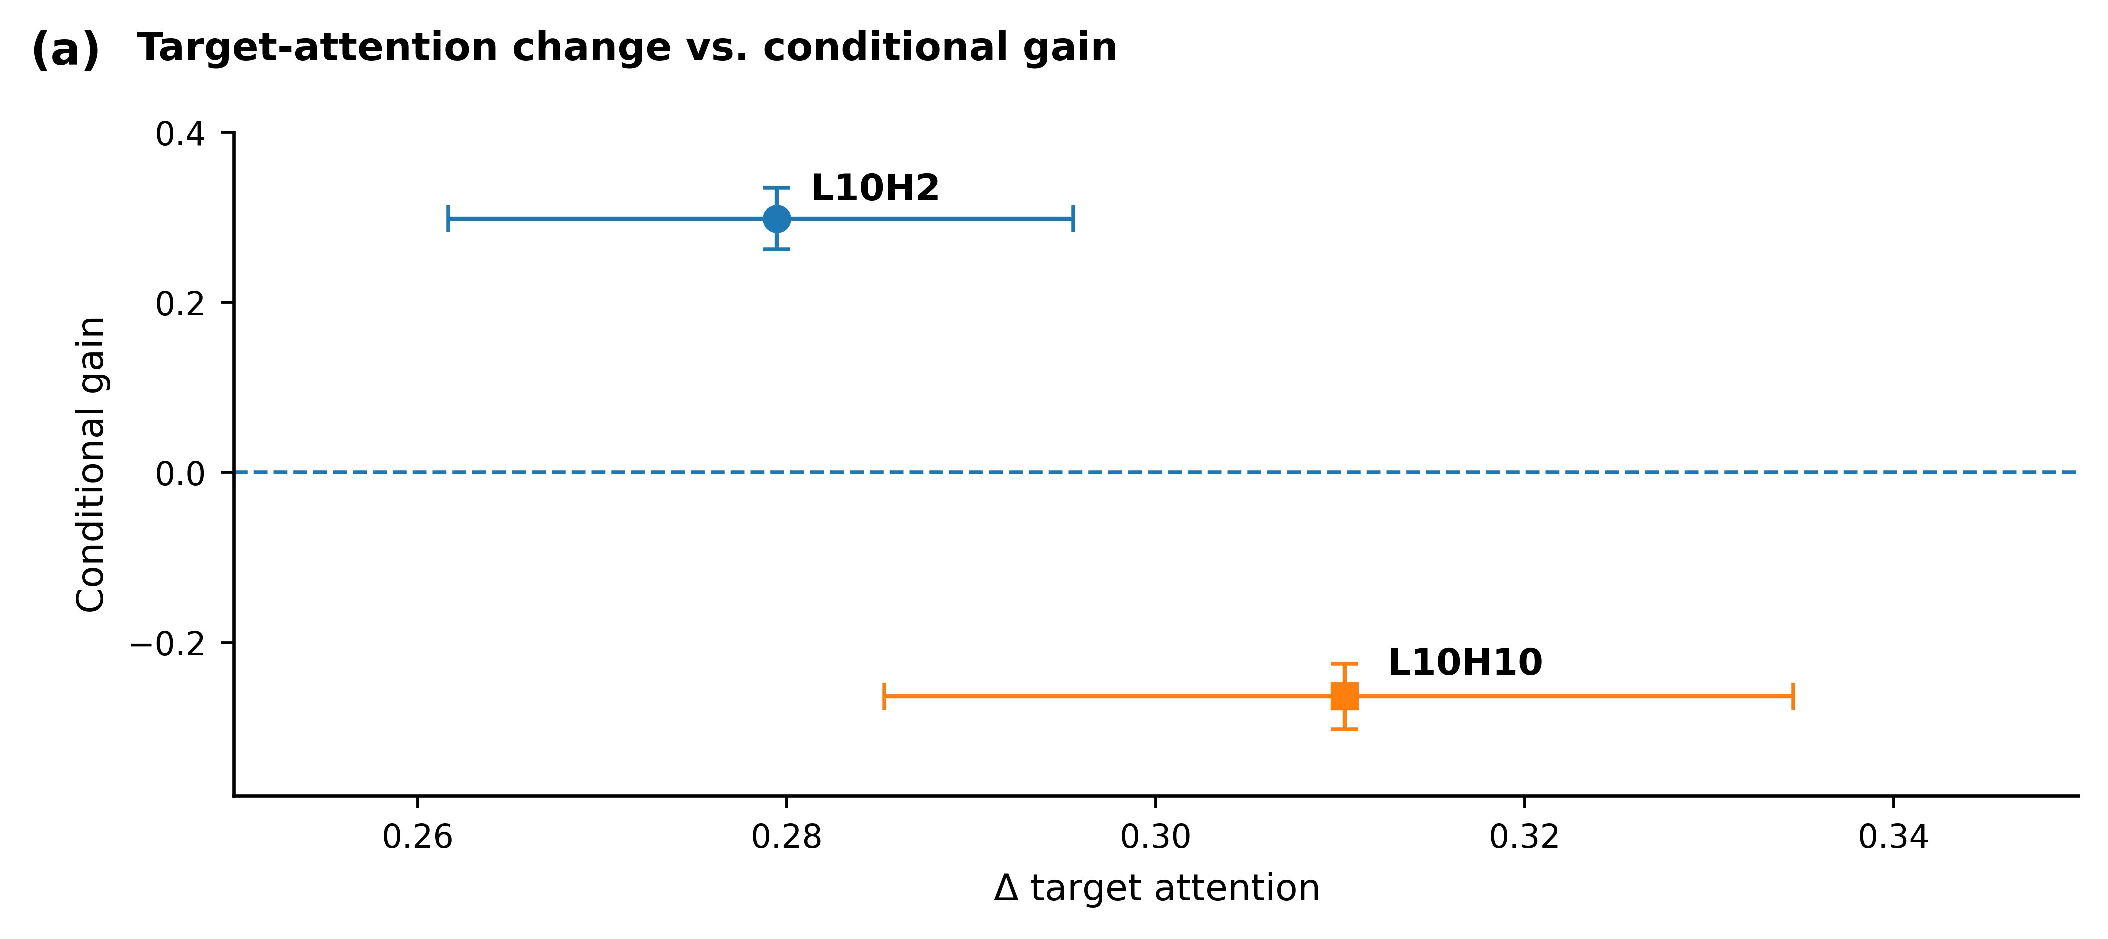
\includegraphics[width=0.95\textwidth]{figures/Fig4a.pdf}
\caption{\textbf{Target-attention adaptation is not sufficient for positive functional recruitment in GPT-2 IOI.}
(a) L10H2 and L10H10 both increase attention to the indirect-object target after ablation of the canonical primary Name Movers, but their conditional gains have opposite signs: L10H2 becomes more causally useful whereas L10H10 becomes less useful on the broad canonical distribution.
Points are exact balanced means; horizontal and vertical intervals are hierarchical 95\% bootstrap confidence intervals over the canonical template design.}
\label{fig:gpt2-attention-recruitment}
\end{figure*}


\subsection{What changes account for the GPT-2 response?}\label{sec:gpt2-fali}

For positively recruited L10H2, the coarse SCORE contribution is positive ($\Phi_{\mathrm{SCORE}}=0.445$), while value contributes approximately zero and surrounding context contributes negatively ($\phi_C=-0.146$). Within SCORE, the dominant pattern is target-positive and rival-negative: $\phi_T=0.783$ (95\% CI $[0.722,0.838]$) and $\phi_R=-0.341$ ($[-0.372,-0.311]$), with $\phi_O=0.0039$. The directional pattern holds in every seed and every canonical stratum, and remains when the legacy-overlapping template is excluded.

L10H10 exhibits the same fine-score signs despite its negative functional gain: $\phi_T=0.329$ ($[0.300,0.355]$) and $\phi_R=-0.126$ ($[-0.139,-0.113]$). Its positive SCORE contribution ($0.206$) is outweighed by a substantially negative surrounding-context contribution ($\phi_C=-0.471$). Figure~\ref{fig:gpt2-attention-recruitment}b--c shows both the fine score decomposition and the coarse score/value/context accounting.

This comparison is important for interpretation. A target-positive/rival-negative score reorganization is not synonymous with recruitment: it can occur in a head whose net causal usefulness decreases. Recruitment is defined by the output-grounded candidate effect; FALI then explains how the cross-state change is allocated under the intervention game. The same-layer controls L9H7 and L9H0 provide the complementary architectural case: their candidate score/value states do not change across the primary intervention, so their measured cross-state changes are assigned to surrounding context up to numerical precision.

\begin{figure*}[!t]
\centering
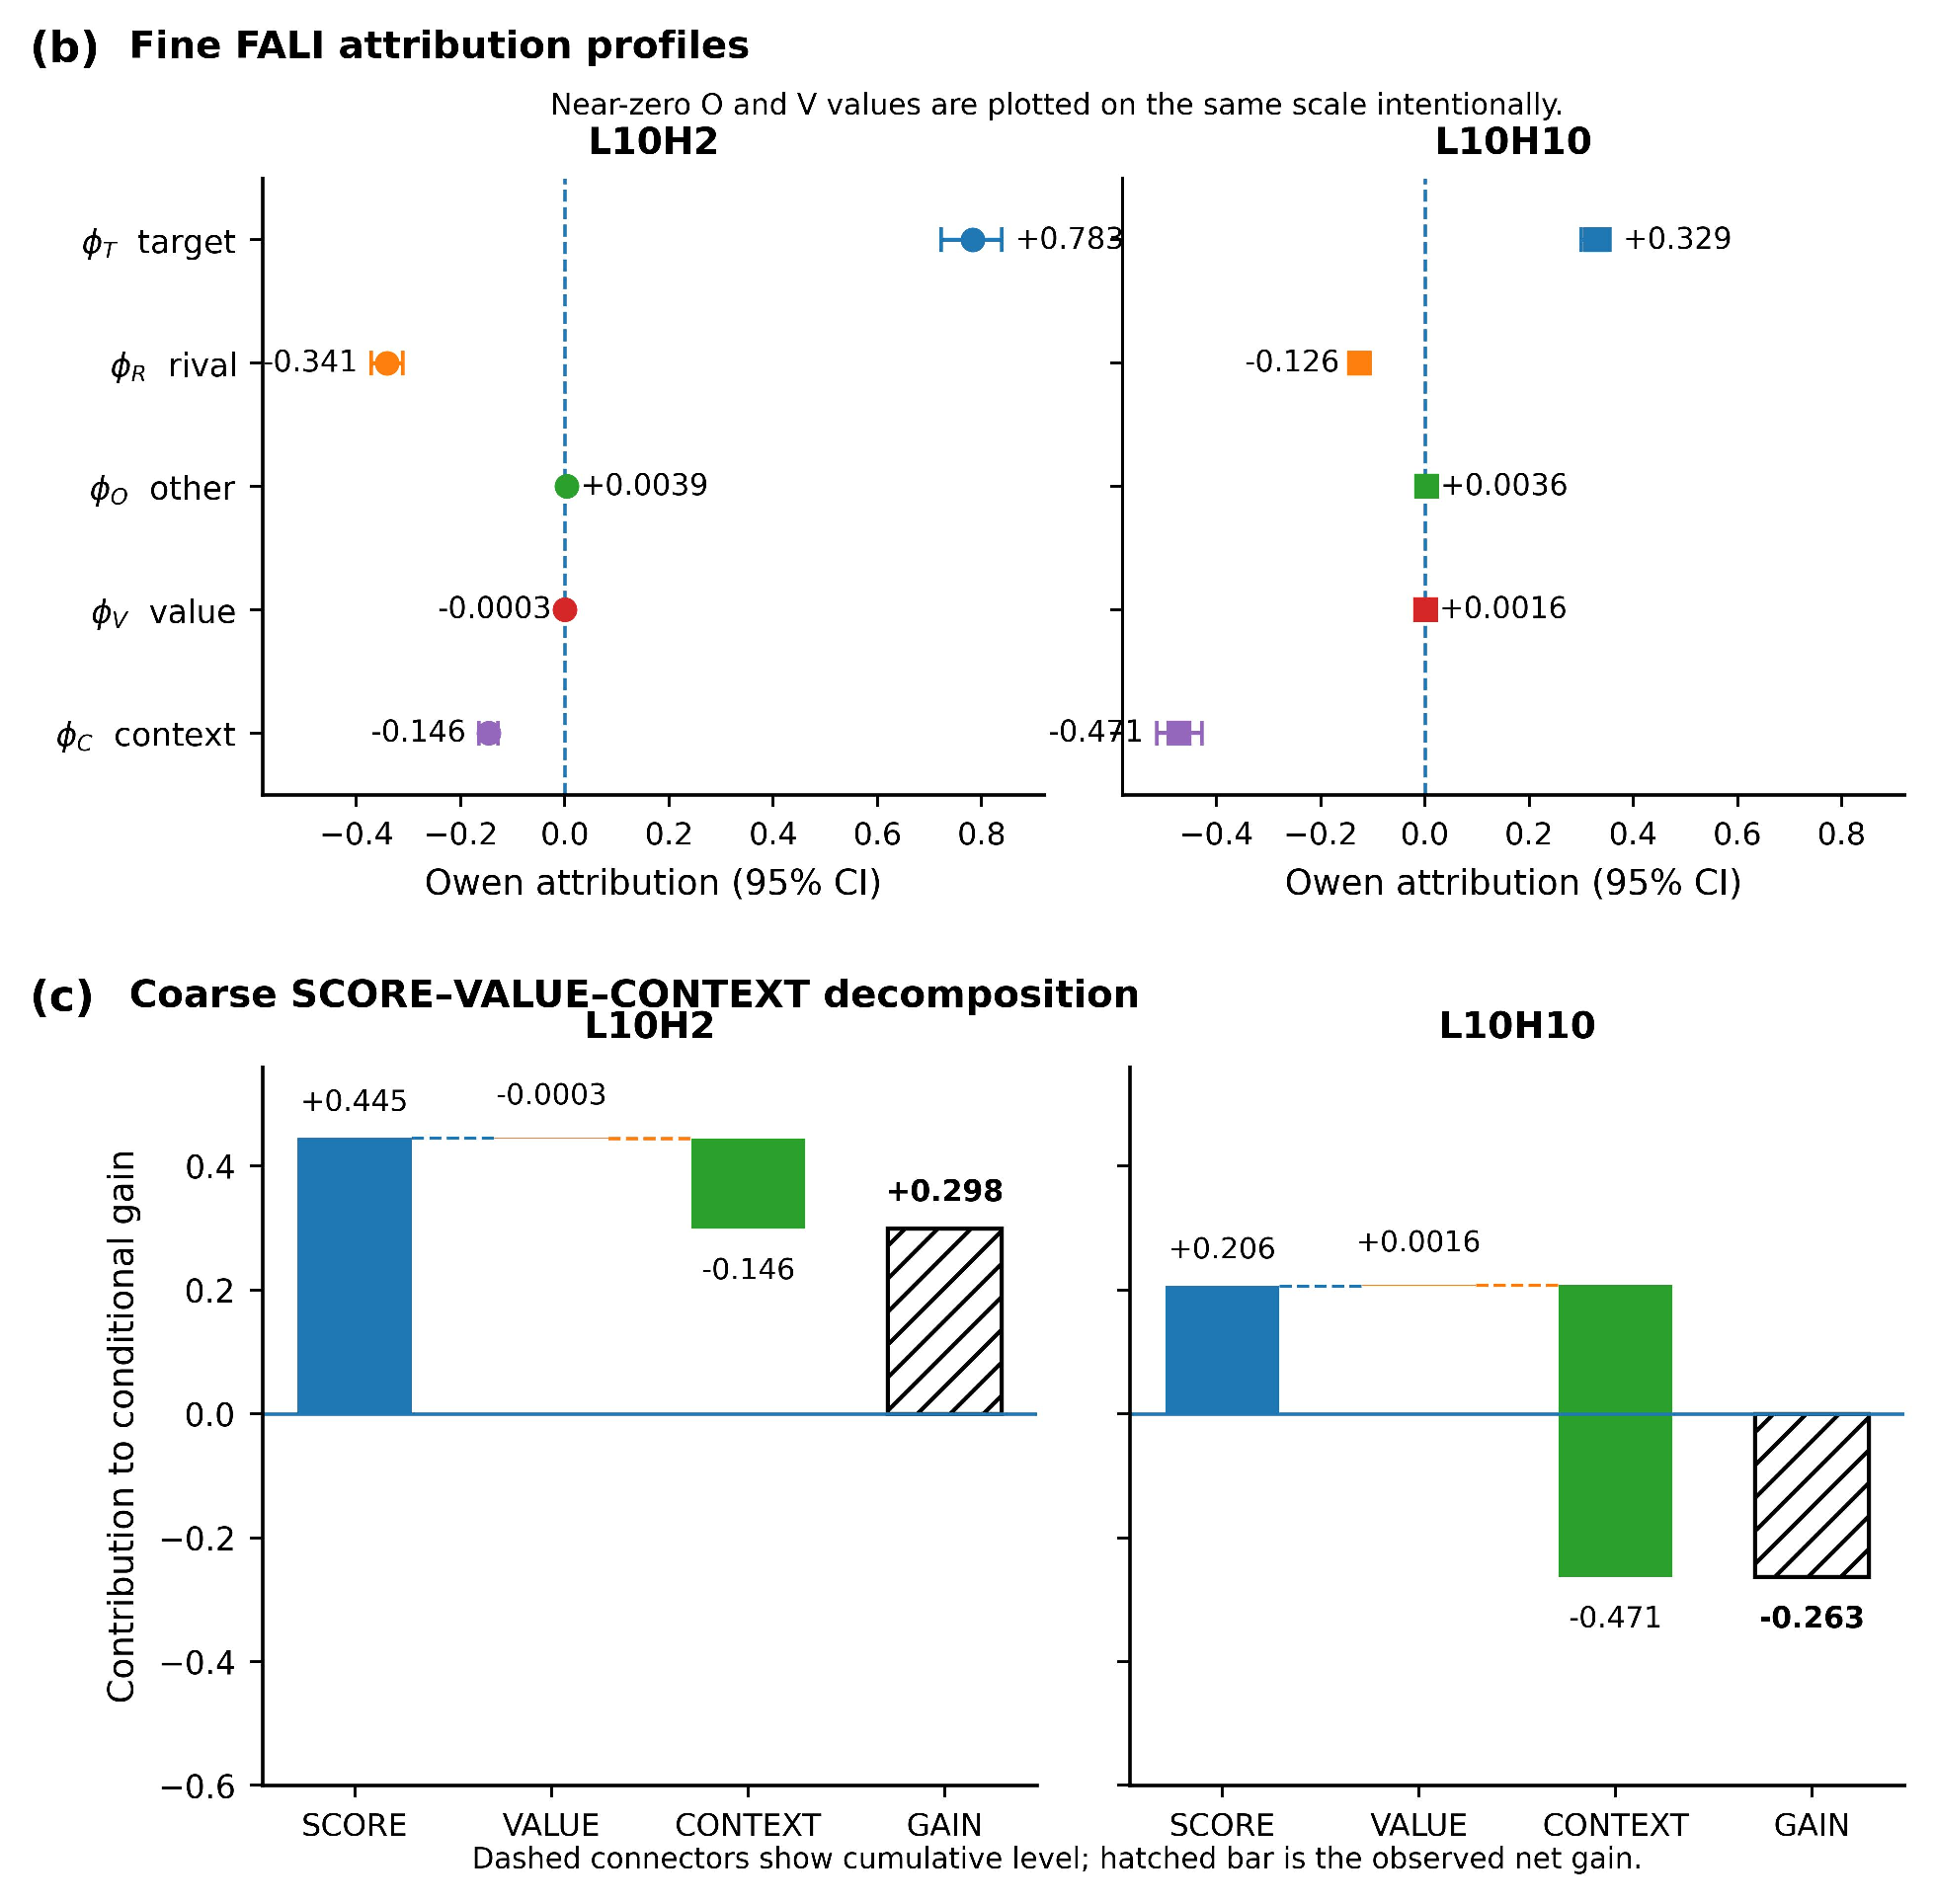
\includegraphics[width=0.92\textwidth]{figures/Fig4bc.pdf}
\par\smallskip
\noindent\textbf{Figure 4 (continued).} Fine and coarse FALI decomposition in GPT-2 IOI.
(b) Both L10H2 and L10H10 have positive target-score and negative rival-score contributions under the canonical FALI game; $O$ and $V$ remain near zero on the same plotted attribution scale.
(c) The coarse score/value/context decomposition explains why the same fine-score sign pattern does not imply the same functional response: L10H10 retains a positive SCORE contribution, but a substantially negative surrounding-context contribution outweighs it and produces a negative conditional gain.
Points are exact balanced means; intervals in panel (b) are hierarchical 95\% bootstrap confidence intervals. The context factor $C$ denotes surrounding-network/context contribution under the specified intervention game and is not a uniquely localized downstream mechanism.
\end{figure*}


\section{Ablation and Gauge Robustness}\label{sec:robustness}

\subsection{Intervention robustness}\label{sec:gpt2-robustness}
EF-5 tested matched-mean and matched-resample alternatives to the canonical zero ablation. The preregistered fine channels retained their directions under both schemes, with hierarchical CIs excluding zero and the predicted sign in all 30 strata. Under matched mean, L10H2 had $\phi_T=0.440$, $\phi_R=-0.166$ and L10H10 $\phi_T=0.188$, $\phi_R=-0.0816$; under matched resample the corresponding values were $0.265,-0.0474$ and $0.0858,-0.0150$.

The overall EF-5 gate nevertheless \emph{failed}. Its zero-ablation reference criterion required a positive damage-drop CI, but the observed reference was $-0.319$ with CI $[-0.396,-0.244]$, triggering the preregistered stop condition. We therefore claim robustness only for the fine-channel directions under the tested matched alternatives, not robustness to arbitrary ablations or an overall EF-5 pass.

\subsection{Softmax-gauge sensitivity}\label{sec:gauge}

Raw attention logits are defined only up to a per-query additive constant under softmax, so FALI attributions computed on native logits could in principle depend on that gauge. Native-logit FALI remains the primary analysis. As a reviewer-motivated sensitivity, we apply a \emph{prespecified} row-centering (zero-mean) gauge fix to score tensors before recomputing the same Owen game, using the preregistered protocol frozen at commit \texttt{e60f81a} and the executed analysis recorded at commit \texttt{4313519}.

On GPT-2 IOI (EF-4), the fine-channel signs are preserved under row-centering: L10H2 retains $\phi_T>0$ and $\phi_R<0$ (native means $\phi_T=0.783$, $\phi_R=-0.341$; row-mean means $\phi_T=0.644$, $\phi_R=-0.202$), and L10H10 likewise retains $T>0$, $R<0$ (native $0.329$, $-0.126$; row-mean $0.306$, $-0.103$). On Pythia induction (EF-6), L8H2 retains the reversed pattern $T<0$, $R>0$ (native $\phi_T=-0.144$, $\phi_R=+0.118$; row-mean $-0.047$, $+0.021$). Attribution magnitudes change under the gauge fix---noticeably for Pythia---while coarse SCORE, value, context, and conditional-gain endpoints remain numerically unchanged at recorded precision, as expected when the pure endpoints use native softmax scores.

The supported claim is therefore narrow: \emph{the fine-channel sign conclusions are robust to the prespecified zero-mean gauge sensitivity analysis.} This does not establish complete gauge invariance, magnitude invariance, or that row-centering uniquely resolves representation dependence. Detailed paired tables appear in the supplement.

\section{Cross-Setting Test: Pythia Induction}\label{sec:pythia}

\subsection{Preregistered transfer design}\label{sec:pythia-design}

We preregistered one transfer test of the GPT-2 target-positive/rival-negative pattern using Pythia-160M on repeated-token induction. For offsets $j\in\{8,16,24\}$, the input is $[x_0,\ldots,x_{31},x_0,\ldots,x_j]$, the target is $x_{j+1}$ at final query $q=32+j$, and the FALI target key is $k=j+1$; a matched control replaces the first block with disjoint tokens. The transfer hypothesis predicted $\phi_T>0$ and $\phi_R<0$ for a later head that became more useful after an earlier induction head was removed. Failure of either sign counted against transfer.

Head selection was separated from FALI attribution. Discovery used seed 42 only (128 examples per offset; 384 total) and was forbidden from inspecting FALI attributions. Eligibility required a causally useful primary head and a later candidate with positive conditional effect and gain; the frozen selection rule chose L5H0 as primary and L8H2 as candidate. Confirmation then used seeds 1, 8, and 22, again with 128 examples per offset (1152 total). Estimates balance offsets within seed and seeds equally; 95\% intervals use 10,000 deterministic bootstrap draws within seed--offset cells. The five frozen gates were induction behavior (G0), primary causal importance (G1), positive conditional recruitment (G2), transferred $\phi_T>0$ (G3), and transferred $\phi_R<0$ (G4).

\subsection{Positive recruitment recurs while the fine mechanism reverses}\label{sec:pythia-results}

The held-out cohorts satisfy the behavioral and functional prerequisites. Induction advantage is $14.017$ (95\% CI $[12.280,15.939]$), the L5H0 primary drop is $1.146$ ($[0.887,1.539]$), and L8H2 is positively recruited: conditional effect $0.621$ ($[0.456,0.860]$) and conditional gain $0.486$ ($[0.326,0.722]$). These quantities have the required direction in every confirmation seed and offset, so G0--G2 confirm independently of the fine-score hypotheses. Panel (a) of Fig.~\ref{fig:cross-setting-reversal} shows the shared functional result: conditional gain is positive in both the GPT-2 IOI and Pythia induction cases.

The fine mechanism reverses. FALI gives $\phi_T=-0.144$ (95\% CI $[-0.247,-0.084]$) and $\phi_R=+0.118$ ($[0.058,0.219]$), with the reversed sign in every seed and offset. This is not a near-zero failure: relative to the preregistered absolute score-channel denominator $0.261807$, $|\phi_T|$ and $|\phi_R|$ account for approximately $54.9\%$ and $45.0\%$, respectively. The remaining channels are small for $O$ ($\phi_O=-0.00027$, descriptive) and $V$ ($\phi_V=-0.00210$), while the surrounding-context contribution is positive and large ($\phi_C=0.514$); as elsewhere, $C$ is not interpreted as a uniquely localized external mechanism. Panel (b) of Fig.~\ref{fig:cross-setting-reversal} contrasts the target, rival, and surrounding-context attributions directly with GPT-2 IOI and shows the sign reversal with preregistered confidence intervals.

Accordingly, EF-6 is \textsc{Fail}: G0--G2 confirm, while G3 and G4 do not. No alternate pair, model, task, or threshold was substituted after this outcome. GPT-2 IOI and Pythia induction therefore both contain positive conditional recruitment in the studied cases, but their fine target/rival organizations are opposite. This falsifies transfer of the preregistered GPT-2 fine-score mechanism to the tested Pythia setting; it does not establish that no shared recruitment mechanism exists more generally. Figure~\ref{fig:cross-setting-reversal} therefore separates the shared functional recruitment result from the failed preregistered fine-mechanism transfer.

\begin{figure*}[t]
\centering
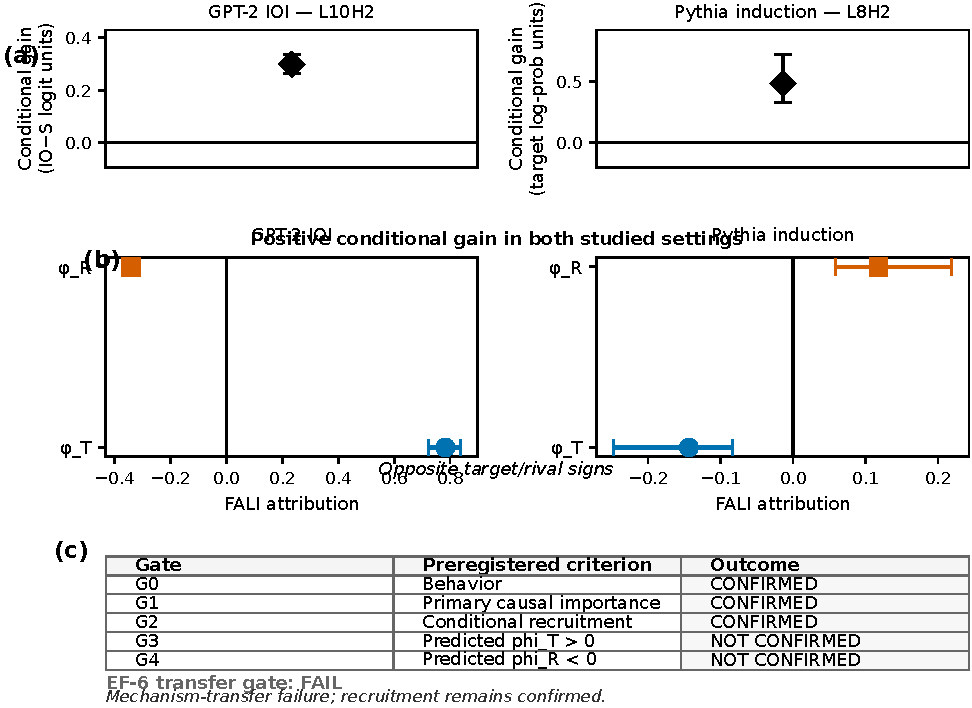
\includegraphics[width=\textwidth]{figures/Fig5.pdf}
\caption{\textbf{Conditional recruitment occurs in both studied settings, while the preregistered fine-score mechanism does not transfer.}
(a) GPT-2 IOI L10H2 and Pythia-160M induction L8H2 both have positive conditional gain after their respective primary interventions. Separate task-specific axes are used because the underlying utility metrics differ; numerical magnitudes should not be compared across tasks.
(b) The observed fine attribution signs reverse: GPT-2 is target-positive/rival-negative, whereas Pythia is target-negative/rival-positive; their surrounding-context contributions also differ in sign. Points are exact balanced means and intervals are the preregistered 95\% bootstrap confidence intervals for each experiment. The Pythia transfer test confirms induction behavior, primary-head importance, and positive conditional recruitment, while the preregistered target-positive/rival-negative fine-mechanism hypotheses are not confirmed. This is a failed mechanism-transfer hypothesis, not a failed recruitment result.}
\label{fig:cross-setting-reversal}
\end{figure*}


\section{Discussion}\label{sec:discussion}

\subsection{A common functional response need not imply a common mechanism}\label{sec:discussion-mechanisms}

The central empirical result is a failed mechanism-transfer hypothesis. GPT-2 IOI L10H2 is positively recruited after removal of the canonical primary Name Movers and has target-positive/rival-negative FALI score contributions; Pythia-160M induction L8H2 is also positively recruited after its primary intervention, but the preregistered fine-score signs reverse. Conditional recruitment therefore occurs in both studied settings while the specific GPT-2 fine-score organization does not transfer.

This distinction matters because \emph{recruitment} names a change in causal usefulness, not the route by which it arises. Conditional-ablation methods can identify components whose importance changes after another component is removed \citep{gong2026coax}, and interaction analyses show that component effects can depend strongly on the rest of the model \citep{vaidyanathan2026curse}. FALI adds a mechanism-resolution step: under one explicit intervention game, two cases meeting the same functional criterion can receive opposite fine-grained score attributions.

GPT-2 also separates visible attention adaptation from recruitment. L10H10 increases target attention and has the same target-positive/rival-negative score pattern as L10H2, yet its broad-canonical conditional gain is negative. Thus neither attention change nor the sign of an individual FALI channel defines recruitment; the output-grounded candidate effect defines the functional response, and FALI allocates its cross-state change. Our evidence is limited to one GPT-2 IOI and one Pythia induction setting, so the reversal does not imply that fine mechanisms generally differ across models or that no shared mechanisms exist elsewhere.

\subsection{Relationship to conditional attribution and patching}\label{sec:discussion-positioning}

FALI is downstream of localization and conditional-importance analysis. Activation/path patching localizes behaviorally relevant activations or paths \citep{goldowskydill2023pathpatching,zhang2024activationpatching,heimersheim2024activationpatching}; CoAx identifies components whose importance changes after perturbing a primary set \citep{gong2026coax}; interaction-aware mediation analysis characterizes dependence on the surrounding network \citep{vaidyanathan2026curse}. FALI instead assumes a selected attention head and target edge, then asks which changes in its score computation, value content, and surrounding context account for the change in output-grounded usefulness.

The method likewise does not claim novelty for separating routing from transported content or for Owen attribution. QK/OV structure and recent causal routing/value decompositions are established \citep{elhage2021mathematical,franco2025attentioncausal,wang2026fewshot}; FALI applies architecture-aligned interventions to a different estimand, the cross-state change in one head's downstream causal contribution, while explicitly including surrounding context. Standard Owen values provide internally consistent interaction allocation under the frozen coalition structure, not an intervention-invariant or unique natural causal decomposition. A practical workflow is therefore: identify a conditionally important component, then use FALI when the scientific question is why that selected attention head's usefulness changed.

\section{Limitations}\label{sec:limitations}

\paragraph{Hypothesis-driven scope.}
FALI requires a selected attention head and a task-relevant target edge or edge set. IOI and repeated-token induction provide clear target coordinates; less structured tasks may require substantial prior circuit analysis. Because the five-factor game evaluates 32 counterfactual cells per example and candidate, FALI is intended for focused mechanism resolution rather than exhaustive whole-model scanning. Candidate or target selection after inspecting FALI results would introduce substantial researcher degrees of freedom, so confirmatory use should freeze these choices prospectively.

\paragraph{Counterfactual hybrids.}
Mixed $T/R/O/V/C$ states need not occur during natural model execution. They answer what the model would do under the specified interchange intervention, not which latent state it would otherwise visit. Representation-level interventions can move computation away from naturally occurring internal distributions \citep{grant2025divergent}; FALI attributions therefore do not identify five independent natural pathways.

\paragraph{Intervention and coalition dependence.}
Attributions depend on the intact and perturbed endpoints, candidate-zero baseline, score partition, and SCORE/VALUE/CONTEXT coalition structure. Owen attribution allocates interactions consistently within that game, but a different defensible intervention or grouping can allocate credit differently. In GPT-2, the target-positive/rival-negative pattern persists under the tested matched-mean and matched-resample alternatives, while the broader preregistered robustness criterion fails because the zero-ablation reference is invalid. The evidence therefore supports only the intervention variants actually tested.

\paragraph{Score representation dependence.}
Fine $T/R/O$ attributions operate on pre-softmax scores, which admit per-row additive gauge freedom. The primary native-logit conclusions retain their signs under a prospectively specified zero-mean row-centering sensitivity, but the magnitudes change, particularly in Pythia. We therefore claim sign robustness to that sensitivity, not general gauge invariance or magnitude invariance.

\paragraph{Coarse context factor.}
$C$ aggregates surrounding computation outside the explicitly supplied candidate score/value state, potentially including other heads, MLPs, residual representations, normalization, and upstream or downstream changes. A large $\phi_C$ assigns credit to this block of the game but does not identify the external component or pathway responsible. Resolving $C$ would require additional hypotheses and interventions.

\paragraph{Empirical scope.}
The substantive evidence covers GPT-2 Small IOI and Pythia-160M repeated-token induction. This is sufficient to falsify transfer of the preregistered GPT-2 target/rival pattern to the tested Pythia setting, but not to characterize recruitment mechanisms across architectures, scales, tasks, or training stages. Prompt-specific circuit results reinforce this distributional caution \citep{franco2026promptspecific}. The present factorization is also attention-head-specific; MLPs, residual features, or distributed mechanisms would require different architecture-aligned factors rather than mechanically reusing $T/R/O/V/C$.

\section{Conclusion}\label{sec:conclusion}

FALI is an output-grounded counterfactual framework for explaining how a selected attention head's causal usefulness changes after a circuit perturbation. It separates target, rival, and other score changes from value content and surrounding-network context, with standard Owen attribution reconciling fine and coarse accounting.

The experiments show why this resolution matters. Attention adaptation need not imply positive recruitment, and positive recruitment need not share one fine mechanism: GPT-2 IOI and Pythia induction both exhibit conditional recruitment in the studied cases, but their preregistered target/rival score contributions have opposite signs. The warranted conclusion is therefore bounded: under explicit intervention semantics, FALI can distinguish mechanistic explanations that a common functional label alone would conflate.


\section*{Acknowledgements}
The authors thank colleagues who provided feedback on earlier drafts of this work.

\section*{Funding}
This research received no external funding.

\section*{CRediT authorship contribution statement}
\textbf{Ronith Sharmila:} Conceptualization, Methodology, Software, Validation, Formal analysis, Investigation, Data curation, Writing -- original draft, Visualization, Project administration.
\textbf{Delen Dursun:} Supervision, Writing -- review \& editing.
\textbf{Rupesh Agrawal:} Supervision, Writing -- review \& editing.

\section*{Data and code availability}
The study uses publicly available pretrained models and programmatically generated experimental datasets. Processed datasets, aggregate result files, preregistration records, and analysis artifacts supporting the reported results will be archived with the accompanying code release. The code required to reproduce the reported analyses will be made publicly available in the project repository and archived in a persistent release.

\section*{Declaration of competing interest}
The authors declare that they have no known competing financial interests or personal relationships that could have appeared to influence the work reported in this paper.

\section*{Declaration of generative AI and AI-assisted technologies in the writing process}
Generative AI tools, including OpenAI ChatGPT and Cursor, were used during manuscript development to assist with literature search support, drafting and editing, code generation and review, figure-layout development, and LaTeX/repository integration. All experimental designs, scientific claims, numerical results, citations, and final manuscript content were reviewed and verified by the authors against the underlying source code, result artifacts, and primary literature. Quantitative scientific figures were produced using deterministic, source-backed plotting workflows. Generative AI tools are not listed as authors and bear no responsibility for the work.

\bibliographystyle{elsarticle-harv}
\bibliography{references}

\section*{Appendix A. Supplementary data}
Supplementary material associated with this article is provided as a separate
supplement PDF and LaTeX source, and will be uploaded as separate Editorial
Manager files.

\end{document}
